	\newpage
\section{Podręcznik użytkownika}  %6
%Opis jak używać programu. Mogą być z zrzut ekranu razem z opisem. 

\subsection{Informacje ogólne od autorów} %6.1

Witamy w naszej aplikacji mobilnej na Androida do biegania, Runly! Ta aplikacja została zaprojektowana, aby pomóc biegaczom śledzić ich treningi, wyznaczać cele i monitorować postępy. Śledzi ona różne pomiary takie jak kroki, czas, prędkość, dystans i spalone kalorie.

\subsection{Wymagania sprzętowe i systemowe} %6.2

Aby korzystać z tej aplikacji, potrzebujesz smartfona lub tabletu z systemem Android w wersji 5.0 lub nowszej, wyposażony w sensor akcelerometra oraz GPS. Będziesz także potrzebować połączenia internetowego, aby uzyskać dostęp do niektórych funkcji, takich jak lokalizacja GPS i wyświetlanie Map Google.

\subsection{Uprawnienia aplikacji}

Aby aplikacja do biegania działała poprawnie, użytkownik będzie musiał nadać jej następujące uprawnienia:

\begin{itemize}
	\item Lokalizacja GPS: To uprawnienie jest wymagane, aby aplikacja mogła uzyskać dostęp do GPS urządzenia i wyświetlić lokalizację użytkownika na mapie,
	\item Licznik kroków: To uprawnienie jest wymagane, aby aplikacja mogła uzyskać dostęp do czujnika licznika kroków urządzenia i śledzić kroki użytkownika wykonane podczas biegu,
	\item Dostęp do Internetu: To uprawnienie jest wymagane, aby aplikacja miała dostęp do Internetu i wyświetlała mapę oraz dane o lokalizacji,
\end{itemize}
Aby przyznać te uprawnienia, użytkownik będzie musiał przejść do ustawień urządzenia i wybrać aplikację. Stamtąd mogą włączyć niezbędne uprawnienia. Należy pamiętać, że niektóre urządzenia z systemem Android mogą poprosić o te uprawnienia podczas pierwszej instalacji aplikacji lub pierwszego użycia danej funkcji. Uwaga: Konkretne kroki przyznawania uprawnień mogą się różnić w zależności od używanego urządzenia i wersji Androida.

\subsection{Jak korzystać z tej aplikacji}

Wyszukaj, pobierz i zainstaluj aplikację Runly ze sklepu Google Play.

\begin{figure}[!htb]
	\centering
	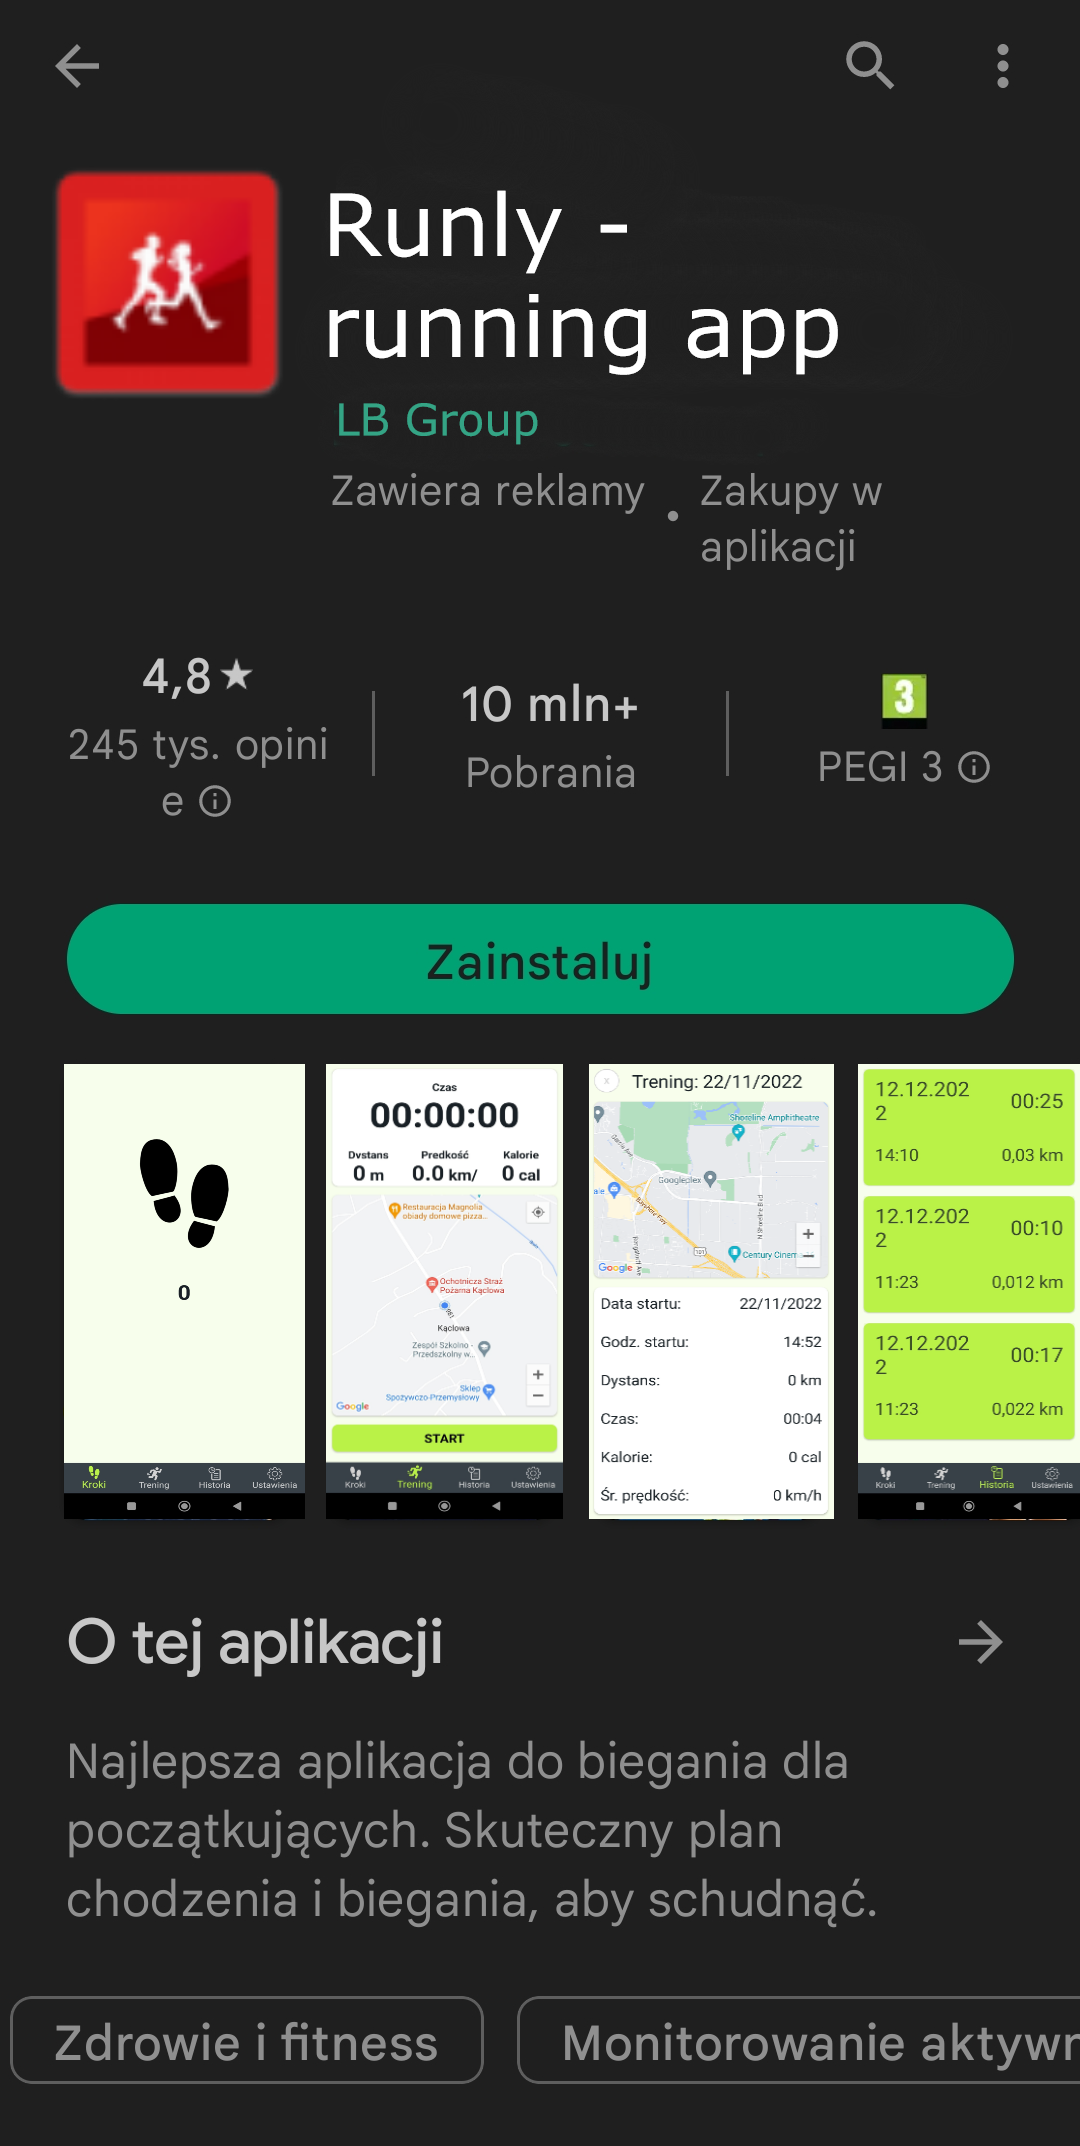
\includegraphics[width=.4\linewidth]{rys/runlyPS.png}
	\caption{Instalacja aplikacji ze sklepu Google Play}
	\label{rys:rysunek001epi}
\end{figure}

Uruchom aplikację.
Wybierz opcję „Rozpocznij trening” z menu głównego.
Rozpocznij trening, a aplikacja będzie śledzić Twoje postępy w czasie rzeczywistym.
Po zakończeniu treningu wybierz opcję „Zakończ trening”, a aplikacja zapisze wyniki.
Aby wyświetlić poprzednie treningi, wybierz opcję „Historia treningów” z menu głównego.
Mamy nadzieję, że korzystanie z tej aplikacji sprawi Ci przyjemność i że pomoże Ci ona osiągnąć Twoje cele fitness!


